%! TeX program = lualatex
\documentclass[../main.tex]{subfiles}
\begin{document} \section{Introduction to random variables}

In a nutshell, a \hlmain{random variable} is a mathematically computable formality to \hlsupp{represent a two-column table} (could have finitely or infinitely many rows) associating each outcome in a sample space \emph{to} a number.  Colloquially, random variables are simply called statistics.

We build some intuition through an example before thinking about formalities. 

\begin{example}[height distribution is a random variable] \label{ex:random-variable-intro}
  Let's collect the height data of some Greek mythical figures and consider the following questions. 

  {\color{main}
    What is the probability of randomly selecting someone whose height is 
    \begin{enumerate}
      \item exactly \(170\) cm?
      \item between \(160\) and \(180\) cm (inclusive)?
      \item at least \(175\) cm?
    \end{enumerate}
  }
  Pay attention to how we use the height data to \hlattn{formulate} each question in the language of probability, i.e., sample space and events. 

  \hfill{}
  \begin{tabular}{l|l}
    Person & Height \\\midrule
    Zeus & \(165\) \\
    Hera & \(152\) \\
    Perseus & \(178\) \\
    Theseus & \(160\) \\
    Athena & \(170\) \\
    Poseidon  & \(170\) \\
    Hades & \(158\) \\
    Helios & \(175\) \\
    Selene & \(167\) \\
    Achilles & \(180\)
  \end{tabular}

\end{example}
\clearpage

Formally, a \emph{random variable}, typically denoted by a capital letter \(X\), is a \emph{function} whose domain is a sample space and whose range is either a set of discrete numbers, e.g., \(\{1,2,3,\ldots\}\), or an interval. 

We need to correctly interpret various notations associated to random variables.
\begin{definition} \label{def:random-variables}
  Let \(X\) be a random variable defined on a sample space \(\Omega\). 

  \begin{itemize}
    \item The notation 
      \[
        {\color{main} X(\text{\hlsupp{the name of an outcome}})}
      \] 
      represents the number associated to \hlsupp{the named outcome} called its \hlmain{\(X\)-statistic}.

      For example, if \(X\) is a random variable recording heights of everybody in our class, then \(X(\underline{\hspace{1in}})\) is \underline{\hspace{1.5cm}} called \underline{\hspace{2in}}.

    \item The notation 
      \[
        X = (\text{some number})
      \] 
      represents \underline{\hspace{2in}} containing outcomes whose \(X\)-statistic is equal to the number on the right-hand side. 

      Consequently, the notation
      \[
        \mathbb{P}(X = (\text{some number}))
      \]
      is the \underline{\hspace{1in}} of randomly selecting an \underline{\hspace{1in}} whose \underline{\hspace{1in}} is \underline{\hspace{2in}}.

    \item The notation (and its variants involving different inequalities)
      \[
        a \le X \le b
      \]
      represents \underline{\hspace{2in}} containing outcomes whose \(X\)-statistic is \underline{\hspace{5in}}.

      Consequently, the notation 
      \[
        \mathbb{P}(a \le X \le b)
      \]
      is the \underline{\hspace{1in}} of randomly selecting an \underline{\hspace{1in}} whose \underline{\hspace{1in}} satisfies \underline{\hspace{2in}}.
  \end{itemize}
\end{definition}

\begin{example}
  Let \(X\) be a random variable representing heights of the class.  Match notations to their verbal descriptions. 

  \begin{multicols}{2}
    \begin{itemize}
      \item \(X \le 180 \text{ cm}\)
      \item \(160 < X \le 180 \text{ cm}\)
      \item \(X = 180 \text{ cm}\)
      \item \(X(\text{Alex})\)
      \item \( X < \infty\)
    \end{itemize}
    \columnbreak
    \begin{itemize}
      \item Everyone whose height is in \((160, 180]\).
      \item Everyone who is at most \(180\) cm tall.
      \item Someone who is exactly \(180\) cm tall.
      \item Everyone who is exactly \(180\) cm tall.
      \item Alex is \(180\) cm tall.
      \item The height of Alex.
      \item The entire sample space.
      \item Empty.
    \end{itemize}
  \end{multicols}
\end{example}

\clearpage
We accumulate some examples before introducing formal definitions.

\begin{example}
  Suppose the sample space is the class population.  Define a random variable \(X\) by associating a person to their \emph{favourite} cupcake flavour.  To simplify the problem, we \hlattn{assume} everyone has exactly one favourite cupcake flavour.

  We represent common flavours using numbers: \(1\) for chocolate, \(2\) for lemon, \(3\) for red velvet, \(4\) for vanilla and \(5\) for none of the above.

  Calculate the following:
  \[
    \mathbb{P}(X = 1) + \mathbb{P}(X = 2) + \mathbb{P}(X = 3) + \mathbb{P}(X = 4) + \mathbb{P}(X = 5) = \underline{\hspace{1in}}.
  \]
  \blanklines{1}

  Is the result surprising? What probability principle from week 6 is at work here?
  \blanklines{15}
\end{example}


\begin{example}
  Cancer are typically classified by stages \(0,1,2,3,4\) with \(0\) being the least severe and \(4\) being the most severe. 

  Suppose \(X\) is a random variable associating cancer patients in a hospital to their stage. An intern arrives with the following probability data. 
  \[
    \mathbb{P}(X \le 1) = 0.2, \quad
    \mathbb{P}(X = 2) = 0.3, \quad
    \mathbb{P}(X = 3) = 0.4, \quad
    \mathbb{P}(X = 4) = 0.5.
  \]

  Does the intern's data make sense? Articulate your reasoning in the language of probability.
  \blanklines{10}
\end{example}

\begin{example}
  Information relevant to a random variable \(X\) recording heights of the class is presented as follows.  
  \[
    \begin{array}{rclcl}
      \mathbb{P}(&X \le 160  &) &=& 0.2  \\
      \mathbb{P}(&X \le 170  &) &=& 0.5  \\
      \mathbb{P}(&X \le 180  &) &=& 0.8  \\
      \mathbb{P}(&X \le 190  &) &=& 0.85 \\
      \mathbb{P}(&X \le 200  &) &=& 0.9  \\
      \mathbb{P}(&X < \infty &) &=& 1 
    \end{array}
  \]

  Fill in the table below. 
    \[
      \begin{array}{rclcl}
        \mathbb{P}(&160 < X \le 170 &) &=& \underline{\hspace{4in}}  \\[2ex]
        \mathbb{P}(&170 < X \le 180 &) &=& \underline{\hspace{4in}}  \\[2ex]
        \mathbb{P}(&180 < X \le 190 &) &=& \underline{\hspace{4in}}  \\[2ex]
        \mathbb{P}(&190 < X \le 200 &) &=& \underline{\hspace{4in}}  \\[2ex]
      \end{array}
    \]
\end{example}
\clearpage

\section{Discrete random variable}

A random variable is discrete if all possible values of \(X(\text{outcome})\) form a discrete set. For all practical intents and purposes, this name is not as important as the two functions associated to them: \emph{probability mass function} (this page) and \emph{cumulative distribution function} (page~\pageref{def:discrete-cdf}).

\begin{definition}[probability mass function]
  The \hlmain{probability mass function} for a discrete random variable \(X\), denoted by \(f_{X}(x)\), is defined by
  \[
    \mathbb{P}(X = x).
  \]
  The subscript of \(f\) indicates the name of the random variable in the context.

  For example, \(f_{X}(0)\) is \(\mathbb{P}(X = 0)\), and \(f_{Y}(-3)\) is \(\mathbb{P}(Y = -3)\).
\end{definition}

\begin{example}
  Describe the probability mass function for the data in Example~\ref{ex:random-variable-intro}.  
  \begin{enumerate}
    \item Introduce appropriate notations.
    \item List all elements in the domain of the probability mass function.
    \item For every number in the domain, describe its output under the probability mass function.
  \end{enumerate}

  \hfill{}
  \begin{tabular}{l|l}
    Person & Height \\\midrule
    Zeus & \(165\) \\
    Hera & \(152\) \\
    Perseus & \(178\) \\
    Theseus & \(160\) \\
    Athena & \(170\) \\
    Poseidon  & \(170\) \\
    Hades & \(158\) \\
    Helios & \(175\) \\
    Selene & \(167\) \\
    Achilles & \(180\)
  \end{tabular}
  \blanklines{15}
\end{example}
\clearpage

The challenge of many problems relating to a probability mass function is knowing what the question asks us to calculate.  \faStar{} An effective problem-solving strategy is to express the event given in the problem using the language of random variables in Definition~\ref{def:random-variables}. 

\begin{example}
  Suppose we have an fair coin. The probability mass function for a random variable \(X\) associating sequences of coin tosses to the number \(k\) of tosses required until a tail appears is
  \[
    f_{X}(k) = (1/2)^{k},  \text{ for integers } k \ge 1.
  \]
  Take for granted that \(f_{X}\) is a legal probability mass function. 


  \begin{enumerate}[wide]
    \item What is the meaning of \(f_{X}(2)\) in the context of this question?
      \blanklines{5}
    \item Describe the event in the question using the language of random variables in Definition~\ref{def:random-variables}. 
      \blanklines{5}
    \item What is the probability that at most \(3\) tosses are required before a tail appears?
      \blanklines{5}
  \end{enumerate}
\end{example}

\clearpage

\begin{definition}[cumulative distribution function] \label{def:discrete-cdf}
  The \hlmain{cumulative distribution function} for a random variable, denoted by \(F_{X}(x)\) is defined by 
  \[
    \mathbb{P}(X \le x).
  \]

  For example, \(F_{X}(2)\) is \(\mathbb{P}(X \le 2)\), and \(f_{Y}(-3432)\) is \(\mathbb{P}(Y \le -3432)\).
\end{definition}

The next example demonstrates the relation between probability mass function and cumulative distribution function for the same random variable. 

\begin{example} \label{ex:random-varialbe-pmf-to-cdf}
  The cumulative distribution function of a random variable \(X\) with range \(\{0,1,2,3,4,5\}\) is given by 

  \begin{minipage}{0.4\textwidth}
    \begin{align*}
      F_{X}(0) &= 0,  \\ 
      F_{X}(1) &= 1/3, \\
      F_{X}(2) &= 5/7, \\ 
      F_{X}(3) &= 4/5, \\ 
      F_{X}(4) &= 1,   \\
      F_{X}(5) &= 1.
    \end{align*}
  \end{minipage}
  \begin{minipage}{0.4\textwidth}
    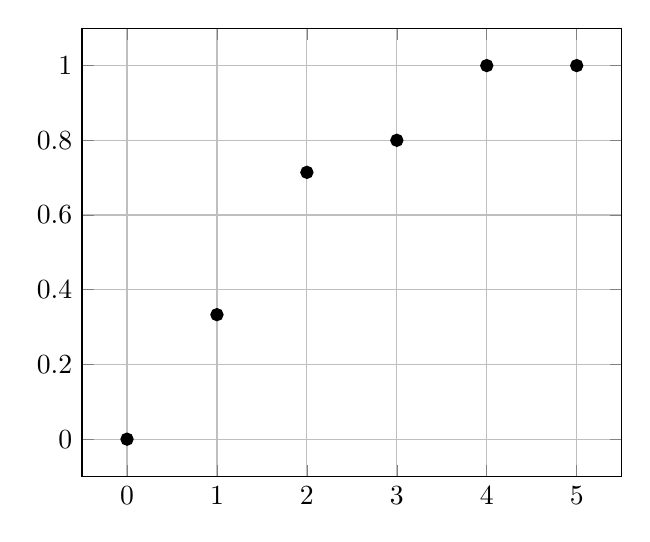
\begin{tikzpicture}
      \begin{axis}[grid=major]
        % \addplot[thick, black, mark=*] coordinates { (0,0) (0,0)};
        % \addplot[thick, black, mark=*] coordinates { (1,0) (1,1/2) };
        % \addplot[thick, black, mark=*] coordinates { (2,0) (2,3/4) };
        % \addplot[thick, black, mark=*] coordinates { (3,0) (3,7/8) };
        % \addplot[thick, black, mark=*] coordinates { (4,0) (4,1) };
        % \addplot[thick, black, mark=*] coordinates { (5,0) (5,1) };
        \addplot[thick, black, mark=*] coordinates { (0,0)};
        \addplot[thick, black, mark=*] coordinates { (1,1/3) };
        \addplot[thick, black, mark=*] coordinates { (2,5/7) };
        \addplot[thick, black, mark=*] coordinates { (3,4/5) };
        \addplot[thick, black, mark=*] coordinates { (4,1) };
        \addplot[thick, black, mark=*] coordinates { (5,1) };
      \end{axis}
    \end{tikzpicture}
  \end{minipage}


  Describe the probability mass function for \(X\). Can you \emph{see} it on the plot?
  \blanklines{10}

  Find the probabilities \(\mathbb{P}(X = 5)\) and \(\mathbb{P}(1 \le X \le 3)\).
  \blanklines{10}
\end{example}

% \begin{definition}[probability density function]
%   The \hlmain{probability density function} \(f(x)\) for a continuous random variable \(X\) is a function \(f(x)\) so that
%   \[
%     \mathbb{P}(a \le X \le b) = \int_{a}^{b} f(x) \;dx.
%   \]
% \end{definition}
\end{document}
